%python
%kelompok 1 D4 TI-3A
%Eka Pratama Putra        1154023
%Deni Braja Astrajingga   1154066
%Shinta Amelia            1154047     
%Luqman Nurfajri	  1154054
%Yoshi Ricowandi Nababan  1154125	
%Copyright (c) 2017 Copyright Holder All Rights Reserved.

\section{Pengertian python}
     
      Menurut beberapa  programmer yang menggunakan bahasa pemrograman python ini, Python merupakan salah satu bahasa pemrograman 
      yang dinamis dan mempunyai sistem manajemen memori yang otomatis Seperti bahasa pemrograman yang dinamis lainnya, Python 
      biasanya digunakan melalui script atau kode-kode meskipun bahasa pemrograman ini lebih banyak dimanfaatkan untuk yang umumnya
      tidak banyak yang menggunakan script. Bahasa Pemrograman Python ini bisa dipakai dan digunakan untuk segala macam kebutuhan 
      dari pengembang-pengembang software atau perangkat lunak dan juga Bahasa Pemrograman Python ini dapat digunakan di berbagai 
      sistem operasi.
      
\section {Sejarah python}
 
      Dalam sebuah artikel oleh Guido van Rossum (berbahasa inggris) yang di terjemahkan menyebutkan bahwa sejarah bahasa pemrograman 
      Python dimulai pada awal 1990 dan diciptakan oleh Guido Van Rossum di Stichting Mathematish Centrum (CWI) Belanda yang merupakan 
      kelanjutan dari bahasa pemrograman ABC.Rilis terakhir Python dari CWI adalah versi 1.2 pada tahun 1995. Kemudian Guido melanjutkan 
      Python pada Corporation for National Research (CNRI) di Virginia. Python versi 1.6 merupakan versi terakhir yang dikembangkan oleh 
      CNRI. Pada tahun 2000, Guido dan pengembang Python berpindah ke BeOpen.com dan hanya merilis satu versi yakni 2.0. Kemudian 
      Guido pindah lagi ke Digital Creations.

	\begin{figure}[ht]
	\centerline{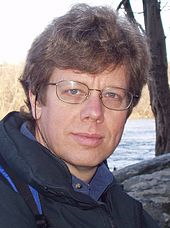
\includegraphics[width=.5\textwidth]{figures/Guido.png}}
	\caption{Guido van Rossum pencipta Python}
	\label{Guido}
	\end{figure}
      
      Gambar \ref{Guido} merupakan foto dari Guido van Rossum yang merupakan pencipta dari python.
      
      Python 3.0 yang juga disebut Python 3000 atau py3k dirilis untuk pertama kali dengan kode yang tidak efisien, dengan dirilisnya pada tanggal 
      3 Desember 2008 dalam periode pengujian yang panjang. Maka, dengan banyak fitur utamanya yang telah dikirim kembali ke Python 2.6 yang cocok ke untuk kembali belakang dan menjadi versi 2.7. 
      
\section {Indentation}
      Dalam penulisan bahasa pemrograman Python, setiap perintah yang masih dalam satu kesatuan diberikan tambahan spasi dari 
      perintah yang ada diatasnya, bukan kurung kurawal atau kata kunci, untuk membatasi blok. Hal ini di sebut juga aturan off-side. 
      Peningkatan indentasi datang setelah perintah tertentu. penurunan identation menandakan akhir blok perintah sebelumnya.

      Contoh perintah bahasa pemrograman python yaitu :
      Perintah perulangan
	  
	  \begin{verbatim}
      while x < 10: 
      	   while y < 10: 
		     print y, 
		     y = y + 1 
	       print x,
	       x = x + 1
	\end{verbatim}

      
\subsection {Fitur dan filosofi}
	Python adalah bahasa pemrograman multi-paradigma: maksudnya pemrograman berorientasi objek dan pemrograman terstruktur 
	yang didukung sepenuhnya, dan ada berbagai fitur bahasa yang mendukung pemrograman fungsional dan pemrograman berorientasi-aspek
	(termasuk metaprogramming dan metode sihir). Banyak model lain yang didukung dengan menggunakan ekstensi, termasuk disain 
	oleh kontrak dan pemrograman logika. 
	Desain Python hanya menawarkan dukungan yang terbatas untuk pemrograman fungsional dalam tradisi Lisp. 
	Bahasa memiliki fungsi peta (), reduce () dan filter (), lengkap untuk daftar, kamus, dan set, serta ekspresi generator. 
	Perpustakaan standar memiliki dua modul (itertool dan functools) yang mengimplementasikan alat fungsional yang dipinjam 
	dari Haskell dan Standard ML\cite {van2007python}.

\section {instalasi python untuk windows}

	Dari sebuah artikel oleh Guido Van Rossum yang telah diterjemahkan, menyatakan bahwa Python Interpreter dan standar library 
	yang tersebar luas tersedia secara bebas dalam berbagai bentuk source atau bentuk biner untuk semua platform utama dari situs 
	Python (www.python.org) dan dapat didownload secara gratis. Situs yang sama juga berisi distribusi dan petunjuk ke bergagai 
	modul, program dan tools Python secara gratis, dan dokumentasi sebagai tambahan. \cite {van1995python}
	di sini penulis artikel menunjukkan instalasi software python yang akan
	digunakan untuk sql injection. Pada dasarnya proses instalasi python tidak jauh berbeda dengan instalasi software pada umumnya
	berikut adalah langkah-langkah instalasi python:

	\begin {enumerate}
	\item
	Langkah pertama adalah klik ganda pada file instalasi python.exe
	kemudian run

	\item
	pilih install for all user kemudian tekan Next. karena tujuannya
	agar aplikasi bisa digunakan oleh setiap user yang ada di pc.
	termasuk guest sekalipun.
			
	\begin{figure}[ht]
	\centerline{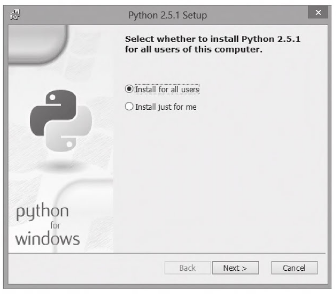
\includegraphics[width=1\textwidth]{figures/awal.PNG}}
	\caption{tampilan awal instalasi}
	\label{awal}
	\end{figure}
	
	gambar \ref {awal} merupakan tampilan awal instalasi app python
	
	\item
	pilih folder tempat instalasi python
	
	\begin{figure}[ht]
	\centerline{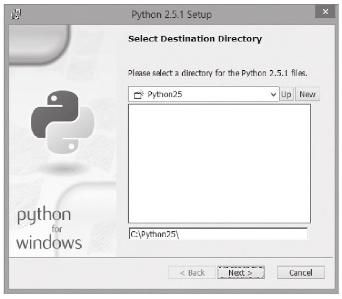
\includegraphics[width=1\textwidth]{figures/folder.PNG}}
	\caption{pilih folder tempat instalasi}
	\label{folder}
	\end{figure}
	
	gambar \ref {folder} tampilan untuk memilih folder instalasi

	\item
	klik next lagi untuk melanjutkan pemasangan

	\begin{figure}[ht]
	\centerline{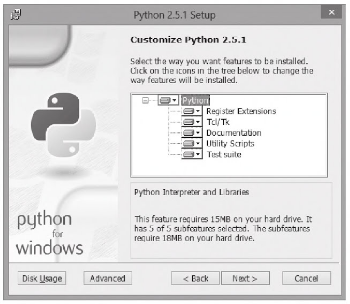
\includegraphics[width=1\textwidth]{figures/komponen.PNG}}
	\caption{komponen yang akan di install}
	\label{komponen}
	\end{figure}
	
	gambar \ref {komponen} merupakan tampilan komponen instalasi python

	\item
	tunggu proses instalasi python beberapa saat
	
	\begin{figure}[ht]
	\centerline{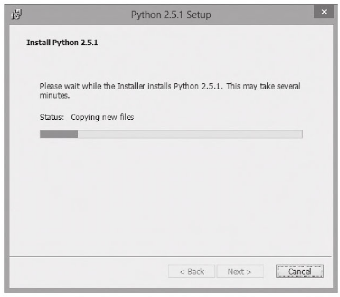
\includegraphics[width=1\textwidth]{figures/proses.PNG}}
	\caption{tampilan proses instalasi}
	\label{proses}
	\end{figure}
	
	gambar \ref {proses} merupakan tampilan proses instalasi

	\item
	jika proses instalasi selesai, klik tombol finish
	
	\begin{figure}[ht]
	\centerline{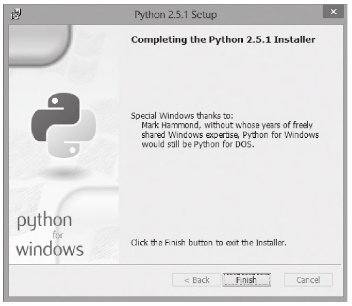
\includegraphics[width=1\textwidth]{figures/selesai.PNG}}
	\caption{tampilan akhir instalasi}
	\label{selesai}
	\end{figure}
	
	instalasi \ref {selesai} software telah selesai dan software python siap digunakan
	
	\end {enumerate}

\subsection {Pemrograman Dalam Bahasa Python}
	Program adalah urut-urutan instruksi untuk menjalankan suatu komputasi. Komputasi dapat berupa matemasis, seperti
	pencarian bilangan prima, persamaan kuadrat, atau yang lainnya. Akan tetapi juga dapat berupa
	pencarian dan penggantian teks dalam dokumen. Instruksi atau perintah atau statement
	pada masing-masing bahasa pemrograman dapat berbeda, namun beberapa instruksi dasar
	secara prinsip hampir disemua bahasa pemrograman sama, seperti :
	
	\begin {enumerate}
	
	\item
	Input
	mengambil data dari keyboard, mouse, file, atau dari device lain.
	\item
	Output
	menampilkan data pada tampilan monitor atau pada device lain.
	\item
	Math
	melakukan operasi dasar matematika seperti penambahan dan perkalian.
	\item
	Conditional
	pemilihan suatu ondisi dan mengeksekusi sesuatu dengan statement selajutnya.
	\item
	Repitisi
	Operasi perulangan.
	
	\end {enumerate}
    
  	Masih banyak hal lain yang belum tercakup diatas, namun program-program bagaimanapun kompleksnya pasti akan terdiri
   	kumpulan intruksi-intruksi di atas.
	Pemrograman merupakan proses yang kompleks yang memungkinkan terjadi kesalahan.
	Berbagai macam kesalahan dapat terjadi dalam pemrograman dinamakan bug. Sedangkan proses pencarian kesalahan dinamakan
	debugging. Dalam pemrograman, kesalahan dapat dibagi menjadi tiga macam, yakni kesalahan sintaks (syntax error), kesalahan run-time (run-time error)
	dan kesalahan dalam pemrograman dapat menjadikan pencarian kesalahan lebih cepat.
	
	\begin {enumerate}
	
	\item
	Kesalahan Sintaks
	   Python hanya dapat dieksekusi jika dan hanya jika program tersebut sintaksnya telah sepenuhnya benar.
	   jika tidak, maka proses akan berhenti dan memberi pesan kesalahan. Sintaks menunjukkan struktur program dan aturannya.
	   Sintaks dalam bahasa Indonesia bisa diumpamakan sebuah kalimat yang harus diawali dengan huruf besar dan 
	   diakhiri dengan titik. Bila terjadi kesalahan sintaks dalam bahasa, maka beberapa pembacac tidak akan begitu mempermasalahkan, tetapi Python
	   tidak demikian. Python harus ditulis dengan benar tanpa ada satupun kesalahan sintaks.
	
	\item
	Kesalahan Run-time
	   Kesalahan tipe kedua adalah kesalahan run-time. Disebut demikian karena kesalahan ini tidak akan muncul sebelum program dijalankan.
	   Kesalahan ini juga sering disebut exception karena kesalahan ini biasanya menunjukkan sesuatu yang ganjil (dan tidak benar) terjadi.
	
	\item
	Kesalahan Logika 
	   Kesalahan tipe ketiga adalah kesalahan logika atau semantik. Jika terjadi kesalahan tipe ini, program akan tetap berjalan dengan sukses tanpa 
	   pesan kesalahan, namun tidak menjalankan program dengan benar atau tidak menjalankan program sesuai dengan
	   maksud yang diinginkan pemrogram.
	
	\end {enumerate}
	
\subsection {methods}
	Metode pada objek adalah fungsi yang melekat pada kelas objek; Contoh sintaks.Metode (argument) adalah untuk metode dan fungsi normal, 
	yang sintaksis untuk Class. Method (contoh, argument). Metode Python memiliki selfparameter yang akurat untuk mengakses data contoh, 
	berbeda dengan diri tersirat pada beberapa bahasa pemrograman berorientasi objek lainnya (misalnya Java, C ++ atau Ruby). 
	
\subsection {typing}
	Python menggunakan bebek mengetik dan telah mengetikkan benda tapi nama variabel untyped. Ketik kendala tidak diperiksa pada waktu kompilasi; Sebaliknya, operasi pada objek mungkin gagal, menandakan bahwa
	Benda yang diberikan bukan tipe yang sesuai. Meski dengan ketahasiaan mengetik, Python sangat kuat diketik, melarang operasi yang tidak didefinisikan dengan baik (misalnya, menambahkan nomor ke a
	string) daripada diam-diam mencoba untuk memahami mereka. Python memungkinkan pemrogram untuk menentukan jenis mereka sendiri menggunakan kelas, yang paling sering
	digunakan untuk pemrograman berorientasi objek. Contoh kelas baru dibuat dengan memanggil kelas (misalnya, SpamClass () atau EggsClass ()), dan kelasnya sendiri
	contoh tipe metaclass (sendiri merupakan contoh dari dirinya sendiri), memungkinkan metaprogramming and reflection. Sebelum versi 3.0, Python memiliki dua jenis kelas: old-style dan gaya baru. Gaya lama
	kelas dieliminasi dengan Python 3.0, membuat semua kelas bergaya baru. Dalam versi antara 2.2 dan 3.0, kedua jenis kelas bisa digunakan. Sintaks dari kedua gaya adalah sama, yaitu
	Perbedaannya adalah apakah objek kelas diwarisi dari, secara langsung atau tidak langsung (semua gaya baru kelas mewarisi dari objek dan merupakan contoh tipe).
      
\subsection {mathematics}
	Berbeda dengan beberapa bahasa pemrograman lainnya, pembagian bilangan bulat didefinisikan sebagai istilah bulat (round) menuju minus tak terhingga. 
	Oleh karena itu 7 // 3 adalah 2, tapi (-7) // 3 adalah -3. Ini seragam dan tetap: misalnya, ini berarti bahwa persamaan (a + b) // b == a // b + 1 selalu benar, 
	sedangkan dalam bahasa seperti C, (-6 + 7) / 7 = = -6 / 7. Ini juga berarti bahwa persamaan b * (a // b) + a\% b == a berlaku untuk nilai positif dan negatif dari a. Namun, menjaga keabsahan persamaan ini berarti bahwa sementara hasil dari\% b seperti yang diharapkan, pada interval setengah terbuka [0, b), di mana b adalah bilangan bulat positif, 
	ia harus berbaring dalam interval (b , 0] ketika b negatif.
	Python menyediakan fungsi bulat untuk pembulatan pelampung ke bilangan bulat. Versi sebelum 3 digunakan round-away-from-zero: round (0.5) adalah 1.0, round (-0.5) adalah -1.0. [45] Python 3 menggunakan round-to-even: round (1,5) adalah 2.0, round (2.5) adalah 2.0. [46] Desimaltype / class dalam module decimal (sejak versi 2.4) memberikan representasi numerik yang tepat dan beberapa mode pembulatan.
	Python memungkinkan ekspresi boolean dengan beberapa hubungan kesetaraan dengan cara yang konsisten dengan penggunaan umum dalam matematika. Misalnya, ekspresi a <b <c menguji apakah a kurang dari b dan b kurang dari c. Bahasa yang diturunkan dari C menafsirkan ungkapan ini secara berbeda: di C, ungkapan pertama akan mengevaluasi sebuah <b, menghasilkan 0 atau 1, dan hasilnya kemudian akan dibandingkan dengan c.

\subsection {Pernyataan dan Arus Kontrol}
	Pernyataan Python antara lain :

	\begin {enumerate}
	\item
	Pernyataan if, yang secara kondisional mengeksekusi satu blok kode, bersama dengan yang lain dan elif (kontraksi yang lain-jika).
	\item
	Untuk pernyataan, yang mengulangi objek yang berulang-ulang, menangkap setiap elemen ke variabel lokal untuk digunakan oleh blok terlampir.
	\item
	Pernyataan sementara, yang mengeksekusi satu blok kode selama kondisinya benar.
	\item
	Pernyataan percobaan, yang memungkinkan pengecualian diajukan di blok kode terlampir untuk ditangkap dan ditangani oleh pengecualian; Ini juga memastikan bahwa kode pembersihan di blok akhirnya akan selalu dijalankan terlepas dari bagaimana blok tersebut keluar.
	\item
	Pernyataan kelas, yang mengeksekusi satu blok kode dan menempelkan namespace lokal ke kelas, untuk digunakan dalam pemrograman berorientasi objek.
	\item
	Pernyataan def, yang mendefinisikan suatu fungsi atau metode.
	\item
	Pernyataan dengan (dari Python 2.5), yang menyertakan blok kode di dalam manajer konteks (misalnya, mengakuisisi alock sebelum blok kode dijalankan, dan melepaskan kunci setelahnya).
	\item
	Pernyataan kelulusan, yang berfungsi sebagai PDN. Secara sintaktis diperlukan untuk membuat blok kode kosong.
	\item
	Pernyataan tegas, digunakan saat melakukan debug untuk memeriksa kondisi yang seharusnya diterapkan.
	\item
	Pernyataan hasil, yang mengembalikan nilai dari fungsi generator. Dari Python 2.5, yield juga merupakan operator. Formulir ini digunakan untuk menerapkan coroutines.
	\item
	Pernyataan impor, yang digunakan untuk mengimpor modul yang fungsi atau variabelnya dapat digunakan dalam program saat ini.
	Python tidak mendukung pengoptimalan panggilan ekor atau kelanjutan kelas satu, dan menurut Guido van Rossum, tidak akan pernah. 
	\end {enumerate}
	Namun, dukungan yang lebih baik untuk fungsionalitas mirip coroutine disediakan di 2,5, dengan memperluas generator Python. 
	Sebelum 2.5, generator adalah pemicu malas; Informasi dilewatkan secara tidak sadar dari generator. Seperti Python 2.5, adalah mungkin 
	untuk menyampaikan informasi kembali ke fungsi generator, dan seperti pada Python 3.3, informasi dapat melewati beberapa tingkat tumpukan.

